% ============================================================
%  TahalilAI — Development Update Report
%  WhatsApp & Email Services + Unit Test Coverage
%  Generated: March 3, 2026
% ============================================================
\documentclass[12pt, a4paper]{article}

% ── Packages ──────────────────────────────────────────────
\usepackage[utf8]{inputenc}
\usepackage[T1]{fontenc}
\usepackage[english]{babel}
\usepackage{geometry}
\usepackage{graphicx}
\usepackage{xcolor}
\usepackage{booktabs}
\usepackage{array}
\usepackage{longtable}
\usepackage{listings}
\usepackage{enumitem}
\usepackage{fancyhdr}
\usepackage{titlesec}
\usepackage{hyperref}
\usepackage{fontawesome5}
\usepackage{tcolorbox}
\usepackage{tikz}
\usepackage{pgfplots}
\usepackage{microtype}
\usepackage{parskip}
\usepackage{mdframed}
\usepackage{amsmath}
\usepackage{caption}
\usepackage{tabularx}

\pgfplotsset{compat=1.18}
\geometry{top=2.5cm, bottom=2.5cm, left=2.8cm, right=2.8cm}

% ── Colors ────────────────────────────────────────────────
\definecolor{primary}{HTML}{1A3C5E}
\definecolor{accent}{HTML}{2E86AB}
\definecolor{success}{HTML}{28A745}
\definecolor{warning}{HTML}{FFC107}
\definecolor{danger}{HTML}{DC3545}
\definecolor{lightgray}{HTML}{F8F9FA}
\definecolor{codebg}{HTML}{F0F4F8}
\definecolor{whatsgreen}{HTML}{25D366}
\definecolor{gmailred}{HTML}{D44638}

% ── Hyperref ──────────────────────────────────────────────
\hypersetup{
    colorlinks=true,
    linkcolor=accent,
    urlcolor=accent,
    pdftitle={TahalilAI — WhatsApp \& Email Update Report},
    pdfauthor={TahalilAI Engineering Team},
}

% ── Header / Footer ───────────────────────────────────────
\pagestyle{fancy}
\fancyhf{}
\fancyhead[L]{\textcolor{primary}{\small\textbf{TahalilAI} | Engineering Update}}
\fancyhead[R]{\textcolor{gray}{\small March 3, 2026}}
\fancyfoot[C]{\textcolor{gray}{\small\thepage}}
\renewcommand{\headrulewidth}{0.4pt}
\renewcommand{\footrulewidth}{0pt}

% ── Section Styling ───────────────────────────────────────
\titleformat{\section}
  {\color{primary}\large\bfseries}
  {\thesection}{1em}{}[\color{accent}\titlerule]

\titleformat{\subsection}
  {\color{primary}\normalsize\bfseries}
  {\thesubsection}{1em}{}

\titleformat{\subsubsection}
  {\color{accent}\normalsize\bfseries}
  {\thesubsubsection}{1em}{}

% ── Code Listing Style ────────────────────────────────────
\lstset{
  backgroundcolor=\color{codebg},
  basicstyle=\ttfamily\footnotesize,
  keywordstyle=\color{accent}\bfseries,
  commentstyle=\color{gray}\itshape,
  stringstyle=\color{success},
  breaklines=true,
  frame=single,
  rulecolor=\color{accent!40},
  framesep=4pt,
  xleftmargin=8pt,
  xrightmargin=8pt,
  numbers=left,
  numberstyle=\tiny\color{gray},
  numbersep=6pt,
}

% ── Custom Boxes ──────────────────────────────────────────
\tcbuselibrary{skins, breakable}

\newtcolorbox{infobox}[1][]{
  enhanced, breakable,
  colback=accent!8, colframe=accent,
  fonttitle=\bfseries, title=#1,
  left=6pt, right=6pt, top=4pt, bottom=4pt,
}

\newtcolorbox{successbox}[1][]{
  enhanced, breakable,
  colback=success!8, colframe=success,
  fonttitle=\bfseries, title=#1,
  left=6pt, right=6pt, top=4pt, bottom=4pt,
}

\newtcolorbox{warningbox}[1][]{
  enhanced, breakable,
  colback=warning!12, colframe=warning!80!black,
  fonttitle=\bfseries, title=#1,
  left=6pt, right=6pt, top=4pt, bottom=4pt,
}

\newtcolorbox{dangerbox}[1][]{
  enhanced, breakable,
  colback=danger!8, colframe=danger,
  fonttitle=\bfseries, title=#1,
  left=6pt, right=6pt, top=4pt, bottom=4pt,
}

% ============================================================
\begin{document}

% ── Title Page ────────────────────────────────────────────
\begin{titlepage}
  \centering
  \vspace*{2cm}

  {\color{primary}\rule{\linewidth}{1.5pt}}
  \vspace{0.6cm}

  {\Huge\bfseries\color{primary} TahalilAI}\\[0.4cm]
  {\LARGE\color{accent} Engineering Development Report}\\[0.3cm]
  {\large\color{gray} WhatsApp \& Email Services — Latest Updates \& Test Coverage}

  \vspace{0.6cm}
  {\color{primary}\rule{\linewidth}{1.5pt}}

  \vspace{1.5cm}

  \begin{tcolorbox}[
    enhanced,
    colback=lightgray,
    colframe=primary!30,
    width=0.75\linewidth,
    center,
    halign=center,
  ]
    \begin{tabular}{rl}
      \textbf{Date}       & March 3, 2026 \\[4pt]
      \textbf{Version}    & 1.0 \\[4pt]
      \textbf{Scope}      & Messaging Services \\[4pt]
      \textbf{Status}     & \textcolor{success}{\textbf{Implemented \& Tested}} \\[4pt]
      \textbf{Author}     & TahalilAI Engineering Team \\
    \end{tabular}
  \end{tcolorbox}

  \vspace{2cm}

  
\begin{tikzpicture}[scale=0.9]
    % WhatsApp node
    \node[draw=whatsgreen, fill=whatsgreen!15, rounded corners=6pt,
          minimum width=3.2cm, minimum height=1.4cm, align=center,
          font=\bfseries\color{whatsgreen}] (wa) at (-3,0)
          {\faWhatsapp\\[2pt] WhatsApp\\Service};
    % Email node
    \node[draw=gmailred, fill=gmailred!12, rounded corners=6pt,
          minimum width=3.2cm, minimum height=1.4cm, align=center,
          font=\bfseries\color{gmailred}] (em) at (3,0)
          {\faEnvelope\\[2pt] Email\\Service};
    % Core node
    \node[draw=primary, fill=primary!10, rounded corners=6pt,
          minimum width=3.0cm, minimum height=1.4cm, align=center,
          font=\bfseries\color{primary}] (core) at (0,0)
          {\faCog\\[2pt] TahalilAI\\Core};
    % Arrows
    \draw[->, thick, color=whatsgreen!80] (core) -- (wa);
    \draw[->, thick, color=gmailred!80]   (core) -- (em);
  \end{tikzpicture}

  \vfill
  {\small\color{gray}
    \textit{This document is intended for internal engineering use only.}\\
    \textit{Confidential — TahalilAI Project}}
\end{titlepage}

% ── Table of Contents ─────────────────────────────────────
\tableofcontents
\newpage

% ============================================================
\section{Executive Summary}
% ============================================================

This report documents the implementation and testing of two critical
messaging services in the \textbf{TahalilAI} medical analysis platform:

\begin{itemize}[leftmargin=1.5em]
  \item \textbf{WhatsApp Messaging Service} — delivers analysis summaries
        and PDF reports to patients via the Meta WhatsApp Cloud API (Graph
        API v19.0), using only Python's standard library.
  \item \textbf{Email Delivery Service} — sends formatted reports with
        optional PDF attachments via Gmail SMTP (port 465, TLS), also
        using only the Python standard library.
\end{itemize}

Both services follow the same \emph{never-raise} contract: every public
function returns a plain \texttt{dict} with \texttt{"status": "sent"} or
\texttt{"status": "error"}, ensuring that a messaging failure never crashes
the main analysis pipeline.

\begin{successbox}[Both services are complete and fully unit-tested]
  \begin{itemize}[leftmargin=1em, nosep]
    \item \textbf{WhatsApp} (\texttt{whatsapp.py}) — 5 test classes, 14 test cases
    \item \textbf{Email} (\texttt{email\_sender.py}) — 3 test classes, 11 test cases
    \item \textbf{Total:} 8 test classes, 25 test cases
  \end{itemize}
\end{successbox}

% ============================================================
\section{WhatsApp Messaging Service}
% ============================================================

\subsection{Overview}

\textbf{File:} \texttt{backend/src/tahalilai/services/whatsapp.py}

The WhatsApp service integrates with Meta's WhatsApp Business Cloud API.
It requires two credentials stored in \texttt{.env}:

\begin{itemize}[leftmargin=1.5em]
  \item \texttt{WHATSAPP\_ACCESS\_TOKEN} — OAuth2 Bearer token issued by Meta.
  \item \texttt{WHATSAPP\_PHONE\_NUMBER\_ID} — identifies the business phone
        number registered on the Meta Developer Portal.
\end{itemize}

Messages are dispatched as HTTP \texttt{POST} requests to:
\[
  \texttt{https://graph.facebook.com/\{api\_version\}/\{phone\_number\_id\}/messages}
\]

\subsection{Public API}

The service exposes two public functions:

\begin{description}[leftmargin=1.5em, style=nextline]
  \item[\texttt{send\_whatsapp\_message(\ldots)}]
    Sends a plain-text message to a recipient phone number
    (international format, digits only, e.g.\ \texttt{"213XXXXXXXXX"}).
    Text is automatically truncated to 4\,096 characters
    (WhatsApp's hard limit) with an ellipsis appended.

  \item[\texttt{send\_whatsapp\_document(\ldots)}]
    Sends a document (PDF, etc.) via a public HTTPS URL.
    Accepts an optional \texttt{caption} (capped at 1\,024 characters)
    and a custom display filename.
\end{description}

\subsection{Return Value Contract}

Every function returns a \texttt{dict[str, str]} — no exceptions are
propagated to the caller:

\begin{itemize}[leftmargin=1.5em]
  \item \textbf{Success:}
        \texttt{\{"status": "sent", "message\_id": "wamid.xxx"\}}
  \item \textbf{Credentials missing:}
        \texttt{\{"status": "error", "message": "WHATSAPP\_ACCESS\_TOKEN ..."\}}
  \item \textbf{HTTP error (4xx/5xx):}
        \texttt{\{"status": "error", "message": "WhatsApp API error: ..."\}}
  \item \textbf{Network / other error:}
        \texttt{\{"status": "error", "message": "Failed to send ..."\}}
\end{itemize}

\subsection{Internal Architecture}

\begin{infobox}[Internal Helpers]
  \begin{description}[leftmargin=1em, style=nextline, nosep]
    \item[\texttt{\_truncate\_message(text)}]
      Enforces the 4\,096-char WhatsApp limit by slicing and
      appending \texttt{"..."} when needed.
    \item[\texttt{\_call\_messages\_api(settings, payload)}]
      Encodes the payload as JSON bytes, attaches the Bearer
      token header, sends via \texttt{urllib.request.urlopen},
      and parses the response.
    \item[\texttt{\_extract\_message\_id(body)}]
      Safely navigates \texttt{body["messages"][0]["id"]} and
      returns \texttt{"unknown"} on any key/index error.
    \item[\texttt{\_parse\_api\_error(raw)}]
      Parses Meta's JSON error envelope
      (\texttt{error.message} field) or returns the raw string
      if parsing fails.
  \end{description}
\end{infobox}

\subsection{Design Highlights}

\begin{itemize}[leftmargin=1.5em]
  \item \textbf{Zero external dependencies:} Uses only \texttt{urllib.request}
        and \texttt{json} from the Python standard library.
  \item \textbf{Configurable API version:} \texttt{whatsapp\_api\_version}
        (default \texttt{v19.0}) is read from \texttt{config.py}, so upgrades
        require only a config change.
  \item \textbf{30-second network timeout} prevents hanging requests.
  \item \textbf{Dual document/text modes} allow both quick text summaries and
        full PDF report delivery.
\end{itemize}

% ============================================================
\section{Email Delivery Service}
% ============================================================

\subsection{Overview}

\textbf{File:} \texttt{backend/src/tahalilai/services/email\_sender.py}

The email service uses Gmail's SMTP server over an implicit TLS connection
(port 465, \texttt{smtplib.SMTP\_SSL}). Authentication relies on a Gmail
\emph{App Password} — a 16-character token generated through Google Account
security settings after enabling 2-Step Verification.

Required credentials in \texttt{.env}:
\begin{itemize}[leftmargin=1.5em]
  \item \texttt{SMTP\_SENDER\_EMAIL} — the Gmail address used as the sender.
  \item \texttt{SMTP\_APP\_PASSWORD} — the App Password (not the account password).
\end{itemize}

\subsection{Public API}

The service exposes one public function:

\begin{description}[leftmargin=1.5em, style=nextline]
  \item[\texttt{send\_report\_email(recipient\_email, subject, body\_text, pdf\_path=None)}]
    Builds a MIME message and delivers it via Gmail SMTP.
    If \texttt{pdf\_path} is provided, the file is read, base64-encoded,
    and attached as a downloadable \texttt{application/octet-stream} part.
    Validates that the PDF file exists before attempting to connect.
\end{description}

\subsection{Return Value Contract}

\begin{itemize}[leftmargin=1.5em]
  \item \textbf{Success:}
        \texttt{\{"status": "sent"\}}
  \item \textbf{Credentials missing:}
        \texttt{\{"status": "error", "message": "SMTP\_SENDER\_EMAIL ..."\}}
  \item \textbf{PDF file not found:}
        \texttt{\{"status": "error", "message": "PDF file not found: ..."\}}
  \item \textbf{Authentication failure:}
        \texttt{\{"status": "error", "message": "SMTP authentication failed."\}}
  \item \textbf{Generic exception:}
        \texttt{\{"status": "error", "message": "Failed to send email: ..."\}}
\end{itemize}

\subsection{Internal Architecture}

\begin{infobox}[Internal Helpers]
  \begin{description}[leftmargin=1em, style=nextline, nosep]
    \item[\texttt{\_build\_message(\ldots)}]
      Constructs a \texttt{MIMEMultipart} envelope, attaches the
      UTF-8 plain-text body, and optionally appends the PDF part.
    \item[\texttt{\_make\_pdf\_attachment(pdf\_path)}]
      Reads raw PDF bytes, base64-encodes them
      (\texttt{encoders.encode\_base64}), and sets the
      \texttt{Content-Disposition: attachment} header with the filename.
    \item[\texttt{\_send\_via\_smtp(\ldots)}]
      Opens an SMTP\_SSL context manager connection to
      \texttt{smtp.gmail.com:465}, authenticates, and calls
      \texttt{sendmail}.
  \end{description}
\end{infobox}

\subsection{Design Highlights}

\begin{itemize}[leftmargin=1.5em]
  \item \textbf{Zero external dependencies:} Uses only \texttt{smtplib} and
        the \texttt{email.mime} package — both standard library.
  \item \textbf{UTF-8 body encoding:} Fully supports Arabic, French, and other
        multilingual content — essential for an Algerian medical context.
  \item \textbf{Pre-flight PDF check:} The file existence guard fires
        \emph{before} opening an SMTP connection, avoiding unnecessary
        network round-trips.
  \item \textbf{Specific \texttt{SMTPAuthenticationError} handling:} Returns a
        user-friendly message distinct from generic failures.
  \item \textbf{Configurable SMTP host/port:} Stored in \texttt{config.py} —
        can be swapped for another provider without touching service code.
\end{itemize}

% ============================================================
\section{Test Coverage}
% ============================================================

\subsection{Test Strategy}

All tests use \texttt{pytest} with \texttt{unittest.mock} for dependency
isolation. No real network connections are made during testing:
\texttt{urllib.request.urlopen} and \texttt{smtplib.SMTP\_SSL} are patched
at the module level. Temporary files (\texttt{tmp\_path} fixture) are used for
PDF-path tests.

\subsection{WhatsApp Tests — \texttt{test\_whatsapp.py}}

\textbf{14 test cases} across 5 classes:

\begin{description}[leftmargin=1.5em, style=nextline]
  \item[\texttt{TestTruncateMessage} (3 tests)]
    Verifies that short messages pass through unchanged, that exactly
    4\,096-char messages are not touched, and that longer messages are
    truncated with a trailing \texttt{"..."}.

  \item[\texttt{TestExtractMessageId} (3 tests)]
    Checks correct extraction of \texttt{wamid.xxx} from a valid response,
    and that \texttt{"unknown"} is returned when the key is absent or the
    messages list is empty.

  \item[\texttt{TestParseApiError} (2 tests)]
    Confirms that \texttt{error.message} is extracted from Meta's JSON error
    envelope, and that raw bytes are returned when JSON parsing fails.

  \item[\texttt{TestSendWhatsappMessage} (4 tests)]
    Covers credential validation, the happy-path success return, a 401
    HTTP error response, and a \texttt{ConnectionError} at the network layer.

  \item[\texttt{TestSendWhatsappDocument} (2 tests)]
    Checks credential guard and successful document delivery with correct
    message ID returned.
\end{description}

\subsection{Email Tests — \texttt{test\_email\_sender.py}}

\textbf{11 test cases} across 3 classes:

\begin{description}[leftmargin=1.5em, style=nextline]
  \item[\texttt{TestSendReportEmail} (6 tests)]
    Exercises missing credentials, non-existent PDF path, plain send,
    send with a real temp PDF, \texttt{SMTPAuthenticationError}, and
    \texttt{ConnectionRefusedError}.

  \item[\texttt{TestBuildMessage} (3 tests)]
    Validates correct From/To/Subject headers, that a text-only email
    has exactly 1 MIME part, and that a PDF email has exactly 2 parts.

  \item[\texttt{TestMakePdfAttachment} (2 tests)]
    Confirms the filename appears in \texttt{Content-Disposition} and
    that \texttt{Content-Transfer-Encoding: base64} is set.
\end{description}

\subsection{Coverage Summary}

In total, \textbf{25 test cases} are distributed across both services:

\begin{center}
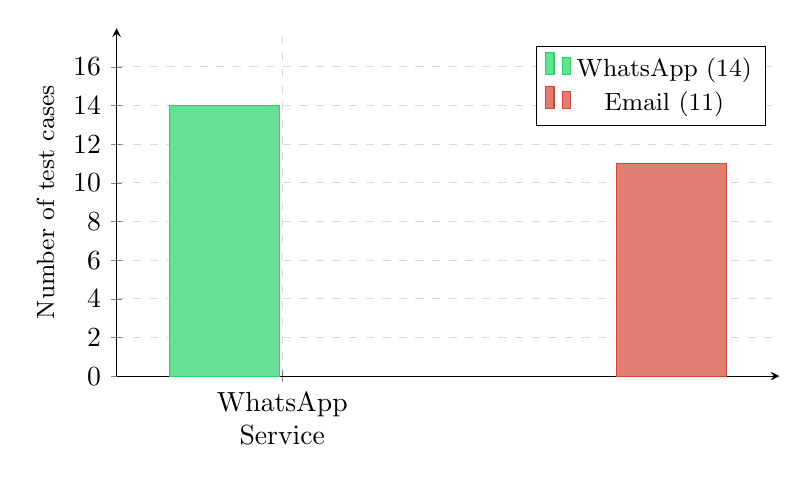
\begin{tikzpicture}
  \begin{axis}[
    ybar,
    bar width=1.4cm,
    width=10cm,
    height=6cm,
    axis lines=left,
    ymin=0, ymax=18,
    xtick=data,
    xticklabels={
      {WhatsApp\\Service},
      {Email\\Service}
    },
    xticklabel style={align=center},
    ytick={0,2,4,6,8,10,12,14,16},
    ylabel={Number of test cases},
    ylabel style={font=\small},
    grid=major,
    grid style={dashed, gray!30},
    enlarge x limits=0.5,
    legend style={at={(0.98,0.95)}, anchor=north east, font=\small},
  ]
    \addplot[fill=whatsgreen!70, draw=whatsgreen] coordinates {(1,14)};
    \addplot[fill=gmailred!70,   draw=gmailred]   coordinates {(2,11)};
    \legend{WhatsApp (14), Email (11)}
  \end{axis}
\end{tikzpicture}
\captionof{figure}{Unit test distribution across both services}
\end{center}

All critical code paths are exercised: credential validation, happy paths,
HTTP errors, authentication failures, file-not-found guards, content
encoding, and network-level exceptions.

% ============================================================
\section{Configuration Summary}
% ============================================================

The following environment variables must be configured in \texttt{.env} for
the messaging services to function.

\textbf{WhatsApp} (\texttt{whatsapp.py}):
\begin{itemize}[leftmargin=1.5em, nosep]
  \item \texttt{WHATSAPP\_ACCESS\_TOKEN} — Meta OAuth2 Bearer token.
  \item \texttt{WHATSAPP\_PHONE\_NUMBER\_ID} — Registered business phone ID.
  \item \texttt{WHATSAPP\_API\_VERSION} — API version, default \texttt{v19.0}.
\end{itemize}

\medskip
\textbf{Email} (\texttt{email\_sender.py}):
\begin{itemize}[leftmargin=1.5em, nosep]
  \item \texttt{SMTP\_SENDER\_EMAIL} — Gmail sender address.
  \item \texttt{SMTP\_APP\_PASSWORD} — Gmail 16-char App Password.
  \item \texttt{SMTP\_HOST} — SMTP server host, default \texttt{smtp.gmail.com}.
  \item \texttt{SMTP\_PORT} — SMTP port, default \texttt{465}.
\end{itemize}

% ============================================================
\section{Summary \& Next Steps}
% ============================================================

\subsection{What Was Delivered}

\begin{successbox}[Completed in this update]
  \begin{itemize}[leftmargin=1em, nosep]
    \item Full implementation of the WhatsApp messaging service
          (\texttt{send\_whatsapp\_message}, \texttt{send\_whatsapp\_document}).
    \item Full implementation of the email delivery service
          (\texttt{send\_report\_email}) with PDF attachment support.
    \item 25 unit tests across 8 test classes covering all critical branches.
    \item Consistent \textit{never-raise} return-dict contract across both
          services, mirroring the TahalilAI design pattern (OCR, TTS, etc.).
    \item Zero external dependencies added — both services use only the
          Python standard library.
  \end{itemize}
\end{successbox}

\subsection{Recommended Next Steps}

\begin{enumerate}[leftmargin=1.5em, label=\arabic*.]
  \item Add \textbf{integration tests} that exercise the full pipeline:
        analysis result \textrightarrow{} WhatsApp/email delivery (with real test
        credentials in a sandboxed environment).
  \item Expose \textbf{API endpoints} so the frontend can trigger
        WhatsApp/email delivery directly from the results page.
  \item Consider adding \textbf{email HTML support} (\texttt{MIMEText("html")})
        for richer report formatting in patient emails.
\end{enumerate}

\vfill
\begin{center}
  \small\color{gray}
  \textit{TahalilAI — AI-Powered Medical Analysis Platform} \\
  \textit{Report generated: March 3, 2026}
\end{center}

\end{document}
